\documentclass{article}
\usepackage[utf8]{inputenc}
\usepackage{amsmath}
\usepackage{amsfonts}
\usepackage{enumitem}
\usepackage{amssymb} 
\usepackage{xcolor}
\usepackage{soul}
\usepackage{todonotes}
\usepackage[margin=2.5cm]{geometry}
\graphicspath{ {./images/} }

\title{Amortized Complexity}
\author{Jin Long Cao}
\date{November 2022}

\begin{document}
\maketitle
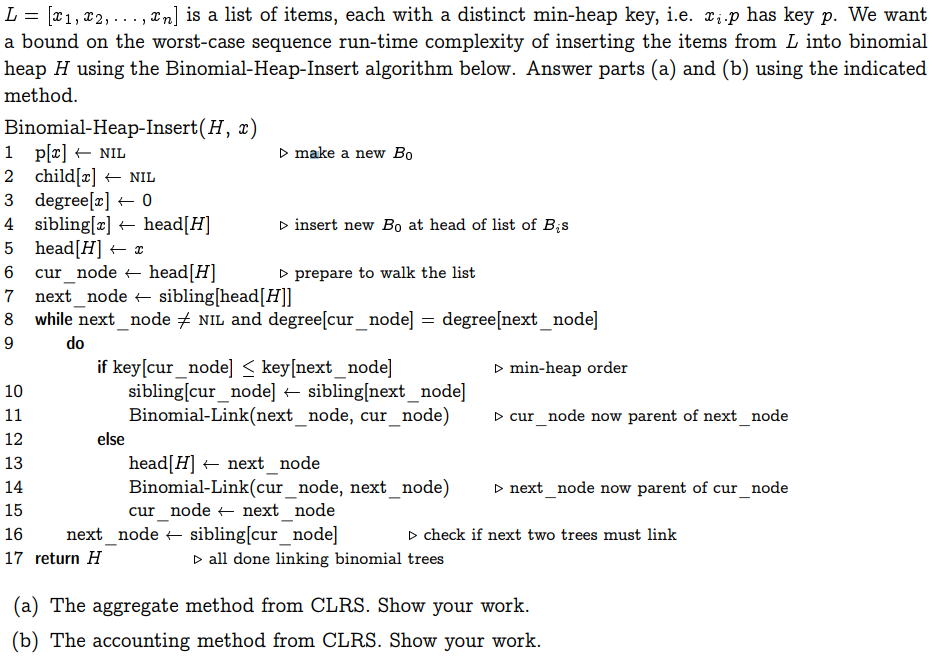
\includegraphics[width=\textwidth]{Amortized Complexity}
\newpage
\section*{Solutions}
Let $L = [x_1, x_2, \dots, x_n]$ be a list of items, each with a distinct priorities ($x_i.p$ has priority $p$). Let $k \in \mathbb{N}$.\\
When inserting into a binomial heap, we need to consider two things. 
\begin{itemize}
    \item MAKE-HEAP(x): return a new heap containing only element x.
    \item UNION($H_1, H_2$): return a new heap containing all elements of heap $H_1$ and $H_2$.
    \begin{itemize}
        \item \textcircled{1} First merge $H_1$ and $H_2$ into $H'$ with binomial trees in ascending order (based on priority).
        \item \textcircled{2} If $H'$ contains 2 $B_k$ adjacent to each other, call them $B_{k_1}$ and $B_{k_2}$, then merge them into a $B_{k+1}$.
        \item \textcircled{3} If there are now 3 $B_{k+1}$ adjacent then we merge the second and third $B_{k+1}$.
    \end{itemize}
\end{itemize}
\underline{Note}: \textcircled{2} may run multiple times until there aren't anymore pairs of $B_k$. \\
For example, consider a binomial heap $H_1$ with binomial trees $B_0, B_1, B_2$. if we insert an element, MAKE-HEAP(x) would creates a new heap with single node $B_0$, then UNION($H_1, B_0$) would merge the two $B_0$ into a $B_1$ (\textcircled{2} ran once), but now we have two $B_1$ which will run \textcircled{2} again resulting in another binomial heap with two $B_2$ which will trigger \textcircled{2} to run again. In this example, \textcircled{2} ran 3 times from inserting one element.
\subsection*{(a) Aggregate Method}
Notice that \textcircled{2} occurs every other time you insert something. Every time you insert something, you create a single node ($B_0$) and then you add it with the rest of your binomial heap. That means every other time you insert something, you'll have two $B_0$ and \textcircled{2} will run (at least once). Also, 
\begin{itemize}
    \item Every fourth insert, we'll have two $B_1$ and \textcircled{2} will have to run again.
    \item Every eighth insert, we'll have two $B_2$ and \textcircled{2} will have to run again. \\
    \vdots
    \item Every $2^k$-th insert, we'll have two $B_{k-1}$ and \textcircled{2} will have to run again.
\end{itemize}
In a sequence of $n$ operations: MAKE-HEAP(x) and \textcircled{1} always run \textbf{($2n$)}, \textcircled{2} will run at least once every other time \textbf{($\frac{n}{2}$)} to combine the two $B_0$. But in total, \textcircled{2} will run in the sequence of $\sum^{k}_{i=1} \lfloor \frac{n}{2^i} \rfloor$. Since we're starting with an empty binomial heap and inserting one element at a time, there won't be any possibility that 3 $B_{k+1}$ are adjacent such that \textcircled{3} will run zero times \textbf{(0)}. Putting it all together, the total number of times each operation runs for $n$ insertion is 
\begin{align*}
    2n + \frac{n}{2} + \frac{n}{4} + \dots + \frac{n}{2^k} &= 2n + n(1 - (\frac{1}{2})^k)\\
    &= 2n + n - n(\frac{1}{2})^k\\
    &< 3n
\end{align*}
Using aggregate method, we can conclude that the total cost of the sequence is $O(n)$ and the amortized cost per operation is $\frac{O(n)}{n}=O(1)$.

% Insert(H, x) inserts node x into heap H. key[x] is filled in. \\
% WC runtime: Theta(lg n) in binomial heap.\\
% n comes b/c union with a n-node binomial heap 
% \\~\\
% Procedure: \\
% make a binomial heap H’ using make-binomial-heap(); allocates and returns an object H’ where head[H’]=NIL? -- theta(1)\\
%  Set parent, child, sibling of x to NIL\\
%  Set degree of x to 0\\
%  Set head[H’] = x; so the binomial heap is just x\\
% Use binomial-heap-union(H, H’) to put them together; Theta(lg n)\\
\newpage
\subsection*{(b) Accounting Method:}
Notice that if a Binomial heap have $2^{k}-1$ nodes (with $k$ binomial trees) and we insert once. Then the binomial heap will have $2^k$ nodes which means it should have only one binomial tree $(B_k)$. To get one binomial tree, UNION will merge $k$ times.\\
\begin{center}
\begin{tabular}{||c c c c||} 
 \hline
 Total nodes & number of merges* & $B_i$ & \\ [0.5ex] 
 \hline\hline
 1 & 0 & $B_0$ & \\ 
 \hline
 2 & 1 & $B_1$ & \\
 \hline
 3 & 0 & $B_0, B_1$ & \\
 \hline
 4 & 2 & $B_2$ & \\
 \hline
 5 & 0 & $B_0, B_2$ & \\ [1ex] 
 \hline
 6 & 1 & $B_1, B_2$ & \\ [1ex] 
 \hline
 7 & 0 & $B_0, B_1, B_2$ & \\ [1ex] 
 \hline
 8 & 3 & $B_3$ & \\ [1ex] 
 \hline
 \vdots & \vdots & \vdots & \\ [1ex] 
 \hline
 n-1 & $\leq\lg (n-1)$ &  & \\ [1ex] 
 \hline
 n & $\leq\lg n$ &  & \\ [1ex] 
 \hline
\end{tabular}\\
*not including the first merge \textcircled{1}
\end{center}

\noindent\underline{Note}: $\nint{x}$ represents rounding to the closest integer to $x$ \\~\\
For MAKE-HEAP(x), it cost 1 to create a singleton heap and it cost another 1 to store an item from $L$ into a binomial heap. Then the amortized cost $= 1 + 1 = 2 = \theta(1)$.\\~\\
For UNION($H_1, H_2$), it cost 1 to just merge $H_1$ and $H_2$ and we would like to save $\nint{\lg n}$ credit in the bank so that we can merge if there are multiple $B_k$ adjacent. From the table above, we know that it will cost less than $\lg n$ so we'll always have enough credit. Then the amortized cost $ = 1 + \lg n = \theta(\lg n)$\\~\\
Combining it together, we now know that the amortized cost of insert $= 2 + 1 + \lg n = \theta(\lg n)$ and can conclude that the bound on the worst-case run-time complexity of inserting the items from $L$ into a binomial heap is $\theta(\lg n)$
\end{document}